%!TEX root = thesis.tex
%\documentclass[10pt,a4paper,onecolumn,twoside,openright]{book}
\let\accentvec\vec
\documentclass[10pt,a4paper,onecolumn,twoside,openright,titlepage]{svmono}
\let\spvec\vec
\let\vec\accentvec
% added by me
\usepackage{siunitx}

\usepackage{amssymb}
\usepackage{caption}
\usepackage{subcaption}
\usepackage[english]{varioref}		% Vario REF \vref
\usepackage{hyperref}			% Clickable links
\usepackage{breakurl}							% Umbrechende URLs
\usepackage{url}
%\usepackage{graphics}
\usepackage{graphicx}							% Graphic support for eps
\usepackage[utf8]{inputenc}		% Input Encoding auf Windows einstellen
\usepackage[T1]{fontenc}					% Umlaute unterstützen
%\usepackage{ams}
\usepackage{textcomp}							% TC fonts
\usepackage{color}
%\usepackage{alltt}								% includes verbatim from text files
\usepackage{lmodern}							% Schriftanpassungen
\usepackage{multicol}							% Mehrere Spalten im Text verwenden
%\usepackage[bottom]{footmisc}			% Fußzeilen
\usepackage{pifont} 							% for fancy bullets
\usepackage{setspace}							% Zeilenabstand
\usepackage{fancyhdr}							% Kopfzeilen
\usepackage{makeidx}							% Index
%\usepackage[english,german]{babel}				%	nationale Datumsformate, etc.
\usepackage[german,english]{babel}
\usepackage{nomencl}							% Erstellt Abkürzungsverzeichnisse
%\usepackage[style=long,border=none,header=plain,cols=2,number=none,hypertoc=true,acronym=false,global=true]{glossary}   %
\usepackage{tabularx}							% Tabellen mit Type X haben automatische minipage mit Zeilenumbruch
\usepackage{multirow}
\usepackage{rotating}             % Rotieren von float elementen
\usepackage{booktabs}							% Tabellen verschönern mit toprule/bottomrule
\usepackage{colortbl}							% farbige Tabellen
\usepackage[numbers, sort]{natbib}								% Naturwissenschaftliches Zitieren
%\usepackage[small, normal, bf, up]{caption2} % Paket für schönere Bildunterschriften
%\usepackage[nottoc]{tocbibind}		% Literaturverzeichnis in Inhaltsverzeichnis aufnehmen
\usepackage{listings} % Programm-Listing
\lstset{language=C}
\usepackage{float}
\usepackage{amsmath}
\usepackage{parskip}
%\usepackage[toc,nonumberlist]{glossaries}
\usepackage[acronym,nomain]{glossaries}
\usepackage[toc]{appendix}
\usepackage{algorithm}
\usepackage{chngcntr}
\usepackage{algpseudocode}
%\usepackage{algorithmic}
\counterwithout{footnote}{chapter}


% The following allows putting comments in the margin: "\marginpar{comment}"
\setlength{\marginparwidth}{1.6in}
\let\oldmarginpar\marginpar
\renewcommand\marginpar[1]{\-\oldmarginpar[\raggedleft\footnotesize \textbf{#1}]{\raggedright\footnotesize \textbf{#1}}}


\fancypagestyle{plain}{										% Redefining the plain style
	\fancyhf{}
	\renewcommand{\headrulewidth}{0pt}
	\renewcommand{\footrulewidth}{0pt}
}


%Kopf- und Fußzeile
\pagestyle{fancy}																		% {fancyhdr}: besetzt Kopf- und Fusszeilen mit definiertem Inhalt
\fancyhf{}																					% clear all header and footer fields
																										% im Stil slanted-shape = geneigt; nouppercase = klein geschrieben
\fancyhead[LE,RO]{\bfseries \thepage}								% LE=left-even + RO=right-odd: \thepage=Seitenzahl
\fancyhead[LO]{\bfseries \nouppercase{\rightmark}}		% LO=left-odd: \rightmark=lower-level sectioning information
\fancyhead[RE]{\bfseries \nouppercase{\leftmark}}		% RE=right-even: \leftmark=higher-level sectioning information
\renewcommand{\headrulewidth}{0.5pt}								% Linie zum Abtrennen der Kopfzeile mit entsprechender Breite
\renewcommand{\footrulewidth}{0pt}									% Linie zum Abtrennen der Fusszeile mit entsprechender Breite (0=keine Linie)
%\setlength\headheight{13.6pt}
\headheight 13.6pt																	% wegen Schriftgröße 11pt muss die Höhe der Kopfzeile vergrößert werden

%\setacronymnamefmt{\gloshort}  % setzt den ersten Wert im Abkürzungsverzeichnis auf die Abkürzung selbst
%\setacronymdescfmt{\glolong: \glodesc}
%\makeacronym
%\newglossarystyle{modsuper}{
%  \glossarystyle{super}
%  \renewcommand{\glsgroupskip}{}
%}
\makeindex
%\makeglossary
\makeglossaries

% Punkte zw. Abkürzung und Erklärung für Abkürzungsverzeichnis
\setlength{\nomlabelwidth}{.20\hsize}
\renewcommand{\nomlabel}[1]{#1 \dotfill}
%\makenomenclature


%\bibliographystyle{unsrtnat}
%\bibliographystyle{unsrt}
\bibliographystyle{acm}
%\bibliographystyle{ieeetr}
\newcommand*{\Mail}[1]{\href{mailto:#1}{\protect\url{#1}}}
\newcommand*{\MailTitle}[2]{\href{mailto:#1@#2}{\protect\url{#1}}}
\newcommand{\keywords}[1]{\par\addvspace\baselineskip\noindent\keywordname\enspace\ignorespaces#1}
\newcommand{\biburl}[2]{\url{#1} (last visited #2)}
\newcommand{\itembf}[1]{\item \textbf{#1}}
\newcommand{\blankpage}{\clearpage{\pagestyle{empty}\cleardoublepage}}

%\def\thechapter{\Alph{chapter}}
%\def\thesection{\arabic{section}}

\onehalfspacing % {setspace}: setzt den Zeilenabstand auf 1,5
% Ränder definieren
\oddsidemargin 1in
\evensidemargin 0.5in

\renewcommand{\arraystretch}{1.5}
\renewcommand{\tabcolsep}{6pt}
\selectlanguage{english}

\definecolor{grey}{rgb}{0.85,0.85,0.85}
\definecolor{hpi_orange}{rgb}{0.88, 0.43, 0.20}
\definecolor{hpi}{rgb}{0.537,0.063,0.165}

\newcommand{\TITLE}{Load Balancing Causal Structure Learning Algorithms in Heterogeneous Computing}
\newcommand{\SUBTITLE}{Lastenverteiltes Kausales Strukturlernen auf Heterogenen Systemen}
\newcommand{\AUTHOR}{Milan Proell}
\newcommand{\EMAIL}{milan.proell@student.hpi.de}
\newcommand{\SUPERVISOR}{Christopher Hagedorn}

\lstset{breaklines=true,
	numbersep=5pt,
	stepnumber=1,
	numbers=left,
	captionpos=b,
	float=htbp,
	basicstyle=\ttfamily\fontsize{9}{12}\selectfont
}
\lstset{frame=tb, aboveskip=0.5cm, belowskip=0.5cm}

\newcommand{\todo}[1]{
  \marginpar{\textbf{\textcolor{hpi}{TODO #1}}}
}

\newcommand{\dummyfig}[2][0.2]{
  \begin{center}
    \fbox{
      \begin{minipage}[c][#1\textheight][c]{0.7\textwidth}
        \centering{#2}
      \end{minipage}
    }
  \end{center}
}

\newacronym{NVRAM}{NVRAM}{non-volatile random-access memory}


\begin{document}
	%!TEX root = thesis.tex
\begin{titlepage}

\thispagestyle{empty}
\begin{center}
%	\vspace{0.1cm}
	\LARGE
	Master's Thesis\\
	\vspace{0.4cm}
	\Huge
    \TITLE{}\\
	\vspace{0.4cm}
	\large
    \SUBTITLE{}\\
	\vspace{0.5cm}
	\LARGE
	\textbf{\AUTHOR}\\
	\normalsize
  \Mail{\EMAIL}\\
	\vspace{0.4cm}
	\small
	Hasso Plattner Institute for IT Systems Engineering\\
	Enterprise Platform and Integration Concepts Chair\\
	\vspace{0.3cm}
	\raisebox{0.5\height}{
\includegraphics[width=3cm]{figures/hpi_logo.pdf}}
	\hspace{1cm}
	
\includegraphics[width=3cm]{figures/Universitaet_Potsdam_logo}\\
	\vspace{0.1cm}
	August-Bebel-Str. 88\\
	14482 Potsdam, Germany\\
	\url{http://epic.hpi.de/}\\
%	\vspace{1.5cm}
\end{center}
%\begin{minipage}[b]{\textwidth}
Supervisors:
\vspace{0.3cm}\\
%\begin{minipage}[b]{0.45\linewidth}
Prof. Dr. Hasso Plattner\\
Dr. Michael Perscheid\\
\SUPERVISOR
\vspace{0.3cm}\\
Hasso Plattner Institute\\
Potsdam, Germany
%\end{minipage}
\vspace{0.4cm}\\
\today
%\end{minipage}
\end{titlepage}

	\pagestyle{empty}
	\cleardoublepage

	\pagestyle{fancy}
	\pagenumbering{roman}
	%!TEX root = ../thesis.tex
\chapter*{Abstract}
Constraint-based causal structure learning algorithms are used to derive causal relationships between variables in observational data. State-of-the-art methods are limited mainly by their long execution time, especially for large and high-dimensional datasets. The performance of constraint-based causal structure learning algorithms such as the PC algorithm is essential for time-dependent and energy-efficient computing. Modern high-performance computing systems mainly consist of conventional processors assisted by specialized processing units such as the graphics processing unit (GPU). Algorithms developed with heterogeneous systems in mind use the system resources and enable full processor utilization. The PC algorithm, which is not designed for heterogeneous systems, has to be adapted to heterogeneous computing. In this thesis, the PC algorithm is parallelized using two different approaches to utilize heterogeneous CPU-GPU systems. The PC algorithm is defined independently from the underlying dataset distribution. Yet, in this thesis datasets are assumed to be multivariate normal distributed. The first approach is a static scheduling approach that balances the work pre-execution, and the second approach is based on workstealing algorithms balancing the split work during execution dynamically. An experimental evaluation of both approaches shows that speedup is achievable even if communication and balancing overhead can limit the parallelization effect. Evaluating the approaches in comparison to the GPU-only accelerated PC algorithm shows that dynamic scheduling on both the CPU and GPU through the workstealing-based approach outperforms the GPU-only solution by 16,5\%. In situations where memory limits are reached on the GPU, speedup factors of up to 6,61 are possible.
% Outline the whole thesis
% motivation etc
% what steps are done
% which results where found
	\clearpage
	%!TEX root = ../thesis.tex
\chapter*{Zusammenfassung}
\hyphenation{kau-sa-le}
Constraint-basierte kausale Strukturlernalgorithmen werden verwendet, um kausale Beziehungen zwischen Variablen in Beobachtungsdaten abzuleiten. Methoden nach dem Stand der Technik sind vor allem durch ihre lange Ausführungszeit begrenzt, insbesondere bei großen und hochdimensionalen Datensätzen. Die Leistungsfähigkeit von constraint-basierten kausalen Strukturlernalgorithmen wie dem PC Algorithmus ist essentiell für zeitabhängiges und energieeffizientes Rechnen. Moderne High-Performance-Computing-Systeme bestehen hauptsächlich aus konventionellen Prozessoren, die von spezialisierten Recheneinheiten wie der Graphics Processing Unit (GPU) unterstützt werden. Algorithmen, die mit Blick auf heterogene Systeme entwickelt wurden, nutzen die Systemressourcen und ermöglichen eine volle Prozessorauslastung. Der PC Algorithmus, der nicht für heterogene Systeme konzipiert ist, muss an das heterogene Computing angepasst werden. In dieser Arbeit wird der PC Algorithmus mit zwei verschiedenen Ansätzen parallelisiert, um heterogene CPU-GPU Systeme zu nutzen. Der PC Algorithmus ist unabhängig von der zugrunde liegenden Datensatzverteilung definiert. In dieser Arbeit wird jedoch davon ausgegangen, dass die Datensätze multivariat normalverteilt sind. Der erste Ansatz ist ein statischer Scheduling-Ansatz, der die Arbeit vor der Ausführung verteilt, und der zweite Ansatz basiert auf Workstealing-Algorithmen, die die aufgeteilte Arbeit während der Ausführung dynamisch verteilen. Eine experimentelle Auswertung beider Ansätze zeigt, dass eine Beschleunigung erreichbar ist, auch wenn Kommunikations- und Balancierungs-Overhead den Parallelisierungseffekt begrenzen können. Die Evaluierung der Ansätze im Vergleich zum rein GPU-beschleunigten PC Algorithmus zeigt, dass das dynamische Scheduling sowohl auf der CPU als auch auf der GPU durch den Workstealing-basierten Ansatz die reine GPU-Lösung übertrifft mit einer um 16,5\% besseren Laufzeit. In Situationen, in denen Speichergrenzen auf der GPU erreicht werden, sind Beschleunigungsfaktoren von bis zu 6,61 möglich.
	%!TEX root = ../thesis.tex
	\glsresetall
	\setcounter{page}{0}
	\setcounter{tocdepth}{4}
	\tableofcontents
	\glsresetall
	\cleardoublepage
	\phantomsection \label{listoffig}
%	\addcontentsline{toc}{section}{List of Figures}
	\listoffigures
	\glsresetall
	\phantomsection \label{listoflst}
	\lstlistoflistings
	\glsresetall
	\newpage
%	\phantomsection \label{listoftab}
%	\addcontentsline{toc}{section}{List of Tables}
%	\listoftables
%	\newpage
	\glsresetall
	\pagenumbering {arabic}
	\setcounter{page}{0}
	%!TEX root = ../thesis.tex
\chapter{Introduction}
In data mining and statistics deriving knowledge from observational data is used to find correlations between variables in the data. Through those correlations data distribution characteristics are found. Correlation does no imply causation, which means that, to understand the data and found correlation thoroughly, causality information has to be gathered.

There are many fields where causal relationships of particular interest. In for example medicine or more specifically genetic research the inference of gene regulatory networks can help estimating causal effects among genes. \cite{rauJointEstimationCausal2013}
% motivation, Relevanz (Anwendungsfall, Daten etc warum Effizienz?)

Moore's Law \cite{mooreCrammingMoreComponents1965} says essentially that transistors placed on an integrated circuit double approximately every two years. This law has been self-fulfilling and can be seen in the real world. Still modern processor development is getting to a physical limit, called the "Power Wall". More transistors, that are more densely placed, with lower voltage, and higher frequencies, produce all together more heat. While cooling performance has its physical limits, the "Power Wall" is hit at some point. To work against this limit, modern processors incorporate multiple cores, that work in parallel.

Multi-core processors can speedup execution, by splitting work and processing that work in parallel. But parallelization has its own limits and converges to an upper bound for any work \cite{amdahlValiditySingleProcessor1967}. While this is specific for the work that is parallelized and there are algorithms and applications specifically desgined to be executed on multiple cores, the upper bound still exists. On of the next logical steps for improving performance and optimizing execution speed is adding specialized processors, tailored for the use case. This is where heterogeneous systems, with heterogeneous processors emerged. The processor best fitting for the work to be done is used and with that the best possible performance is to be expected. But while one processor handles the work, the remaining processors may not be used and additional computing power is lost.

Heterogeneous computing tries to solve the problem of lost computing power in heterogeneous systems by using as many resources of the system as possible. Algorithms and applications are inspected and split into parts that are, given their properties such as parrallelizability, placed onto the different processors. The execution time is reduced, by using multiple specialized processors for the best fitting part of the executed work. A downside of using multiple specialized processors is, that parallelized work almost always needs orchestration and communication between each executing unit. The communication time spent is directly related to the interconnection speed between those executing units.

Modern heterogeneous system interconnects between processors are getting faster. Still the interconnect between processors are one of the slowest connections in a computer. Therefore most heterogeneous computing solutions are limited by their interconnect bottleneck. This bottleneck is such an essential part of heterogeneous computing, that many solutions for heterogeneous systems are even slower while using all of the resources because of the communication overhead. Due to that importance of efficient communication designing heterogeneous algrotihms essentially means solving the communication problem.

In this thesis both the PC algorithm and heterogeneous computing are combined to a efficient PC algorithm variant that can be executed on heterogeneous system to use its resources and get an additional speedup in comparison to the non heterogeneous variant. Using the heterogeneously executed PC algorithm experiments are done to analyze bottlenecks and the efficiency of the solution.

Since many use cases of causal structure learning profit from faster results and dataset can be large scale leading to long execution times, a speedup in execution time is benefitial.

Starting with the theoretical background, basic terminology is introduced. While parallel programming is essential for parallizing algorithms on heterogeneous systems, this topic is covered first. The basics on heterogeneous computing and constraint-based causal structure learning are elaborated in the second part of the background chapter.

After that, in the problem statement chapter, the research question is developed using the acquired terminology and explaining the problem state which is aimed to be solved. 
% Trend hardware? heterogene (vllt dark silicon)
% moores law
% processing speed i limited an does not grow any longer (physics, get too hot when more dense) => dynamic power, power wall
% ILP wall? maybe too detailed
% memory wall (memory speed, and latency limited)
% Dark silicon = next step / power wall 2.0
% - multicore scaling limited as well
% \cite{esmaeilzadehDarkSiliconEnd2011}
% - specialized hardware has potential
% - speedup through using the right processor for the correct task
% - Needs alot more software optimizations
% speedup for what?
% - medical causations => The faster, the better
% - when doing multiple experiments/iterations on data, small speedup can mean alot
% - energy efficiency, by optimal resource usage
% - some processing units are more efficient

% Outline, structure

% Teaser auf problem statement

% Womit muss man sich auseinandersetzen (load balanacing)
	%!TEX root = ../thesis.tex
\chapter{Background}
In this chapter, we will look into heterogeneous computing, heterogeneous systems and the processing units frequently used in such systems. While heterogeneous systems power heterogeneous computing algorithms, they can consist of processing units of all kinds. This thesis focus lies on the central processing unit (CPU) and the graphics processing unit (GPU) as the processing power of a heterogeneous system.
After that, the theoretical background of Causal Structure Learning and the PC-algorithm will be explained, which we will connect to the possible execution on heterogeneous systems.

\section{Heterogeneous Computing}
Heterogeneous computing refers to systems that include conventional as well as specialized processors. Those different processors work cooperatively on the same workload. \cite{shan_heterogeneous_2006} Heterogeneous computing aims to use more than one processing unit of the systems resources and increase the execution effectiveness. Heterogeneity in the computing context refers to different instruction-set architectures (ISA), which means that the processors in this system are heterogeneous in their architecture.
Abstractions can eliminate this heterogeneity for the software developer, but since the heterogeneous processing units have different advantages and disadvantages over another, the developer still has to think about the optimal and efficient usage of the PUs.

Most modern computing systems are heterogeneous and consist of one or more CPUs and one or more GPUs. Therefore a heterogeneous computing approach could be beneficial in their effectiveness for such systems. Both the CPU and the GPU are very different in their architecture and function, so most modern applications only use one of those processors effectively.

CPU-GPU heterogeneous computing approaches are also referred to as hybrid or co-operative execution. In most applications, one of GPU and CPU is called the host, which controls the execution flow and the device that accelerates the execution of the host. Therefore the device is also called the accelerator. In this thesis, both the CPU and the GPU are called processing units (PU) as a term that includes both processors.

\subsection{Central Processing Unit}
The CPU, sometimes also just called processor, is the main instruction executing component of a computer. While modern CPUs introduce parallelism concepts, the primary purpose is still low latency execution of given instructions.
Without those later introduced parallelism concepts, a CPU is only able to execute instructions serially. The ability to run concurrent applications is mainly done by introducing a thread and scheduling concept, which switches those threads periodically using a set of rules. Programs can create such threads using an operating system interface.
Additional performance improvements such as superscalar architectures and instruction pipelines, which can be extended through optimizations such as branch prediction or speculative execution, help support the main goal of the CPU, which is a robust and moderately fast way to run any code.
Modern CPU architectures include instruction set extensions for data-level parallelism, called Single Instruction Multiple Data (SIMD). Those instructions execute operations, which would normally mutate scalar values on vector registers in memory. Those SIMD extensions are common in most modern CPU architectures such as x86\_64 (SSE, AVX) or PowerPC (AltiVec). Mathematical operations benefit of SIMD. Especially in linear algebra, optimized implementations for commonly used vector and matrix operations are implemented in Basic Linear Algebra Subprogram (BLAS) implementations. For realizing an optimal CPU side implementation for this thesis, using BLAS is essential and enables using the CPU resources.
Modern CPUs have multiple so-called cores, which can independently execute instructions and therefore are able to run multiple parallel threads concurrently. This is also called task-level parallelism.
Concurrency between threads that share a common resource introduces another problem. Since there can not be any assumption about the relative speed of those threads, analog interferences are possible. Two threads accessing a resource at nearly the same time can result in a so-called race condition since there is no way to identify the thread that accesses the resource first. To prevent those race conditions, critical sections for safe concurrent access are introduced. At any moment, only one thread is allowed into the critical section shared between the threads. The implementation of a critical section requires atomic read / write behavior.
Such access mechanisms like atomic read/write and critical sections are also crucial in heterogeneous computing, where concurrent memory access of multiple processors can occur.
Frameworks such as OpenMP can help the developer to handle multi-threading and safe concurrency with abstractions of those concepts. OpenMP, a shared/memory parallel programming framework for C/C++ and Fortran framework, helps annotate parallel regions like parallelizable for loops and creates multiple execution threads for those regions using a run-time.
The thesis implementation uses OpenMP for efficiency and parallelism purposes.

\subsection{Graphics Processing Unit}
The GPU handles graphics processing in computer systems. In the beginning video games were the main driver for technical advancements in developing better GPUs. The design of modern GPUs is significantly different from the first GPUs, which had hard-coded pipelines and allow for programming the GPU as a general-purpose processing unit \cite{nickolls_gpu_2010}. For computing graphics, the processing of multiple calculations in parallel is essential. Image and video processing primarily consists of doing the same operation on multiple pixels in parallel. Modern recordings and screens can have up to 8 million or more pixels transformed in real-time (i.e., 60 times per second). Such high throughput rates are only possible with a domain-specific processor such as the GPU that can execute thousands of threads concurrently.
Through the general-purpose programming capabilities of modern GPUs, other problems that require processing large data in parallel can be processed using GPUs. Those capabilities enable scientists and high-performance programmers to boost their parallelizable problems on the GPU.
Another benefit of GPUs in comparison to CPUs is their energy efficiency. GPUs are more energy-efficient than CPUs and are therefore commonly incorporated in high-performance heterogeneous systems such as supercomputers.
Looking into Nvidia GPU architectures such as Volta \cite{NVIDIATESLAV1002017} GPU consists of many Streaming Multiprocessors (SM) that execute multiple thread blocks in parallel. A thread block on Nvidia GPUs is executed by a warp in the SM and that warp incorporates many simple cores that are executed in SIMD groups with a single program counter. A warp on Volta or Pascal Nvidia GPU architecture consists of 32 simple cores which share a common memory region. Programmers of those GPUs have to be aware of those architecture semantics to use the underlying cache, memory, and computation structure optimally. A thread block should, for example, be sized according to the multiple of the size of one warp, even if programmers can decide on other thread block sizes. Volta has 64 Warps per SM, which means a maximum of 2048 threads scheduled concurrently on that SM \cite{noauthor_nvidia_2017}.
Frameworks such as OpenCL or CUDA are application programming interfaces (APIs) created to allow software developers to develop general-purpose applications running on the GPU. CUDA is a super-set language of C/C++ that allows the definition of functions that are run on the GPU and CPU. Annotating functions using \texttt{\detokenize{__device__}}, \texttt{\detokenize{__global__}} and/or \texttt{\detokenize{__host__}} tells the compiler on which processing unit the code can be run. Shared CPU-GPU code is possible, which is well suited for executing code on a heterogeneous system. Other advantages, such as unified memory abstractions for heterogeneous systems, are a deciding factor for using this technology in this thesis.

\begin{lstlisting}[language=C++, caption=Simple CUDA kernel example \cite{EasyIntroductionCUDA2012}, label=lst:kernel]
__global__
void add(int n, float *x, float *y)
{
  int index = threadIdx.x;
  int stride = blockDim.x;
  for (int i = index; i < n; i += stride)
      y[i] = x[i] + y[i];
}
\end{lstlisting}
In listing \ref{lst:kernel} a simple "kernel" function that adds an array to another array in parallel on the GPU is shown. Through the \texttt{\detokenize{__global__}} keyword, the compiler creates machine code suitable for a Nvidia GPU. By invoking this kernel, multiple instances of this function are scheduled in thread blocks on the GPU. The thread id of each invocation is accessed through the variable \emph{threadIdx}, and the number of threads in the block is accessed by \emph{blockDim}. When starting multiple blocks, the block id of the kernel invocation can be accessed by \emph{blockIdx}.
Data passed into the function like the arrays x and y have to is created by CUDA run-time API functions, which handle memory allocation on the GPU \cite{MemoryManagement}.

Nvidia GPUs used as accelerator devices have two different memory spaces. Data structures are created and allocated on the host or CPU memory space. After allocating memory on the GPU, the data has to be moved to the device from the CPU either by a direct transfer or by creating a Unified Virtual Memory system accessible from both CPU and GPU. The CUDA Runtime API enables the programmer to do both. In most cases, a single data transfer is done by allocating with \emph{cudaMalloc} and copying the data to the GPU with \emph{cudaMemcpy}. In the heterogeneous computing context, where data needs to be accessed by both the CPU and the GPU simultaneously, a Unified Virtual Memory (UVM) system helps the programmer with the data management. Since CUDA version 6.0, Nvidia introduced \emph{cudaMallocManaged} which handles necessary data transfer in both directions based on pagination. \cite{gayatri_comparing_nodate} Both the host and device keep track of the pages using a page table. On memory access, missing pages migrate to the correct location.
For performance reasons, the CUDA run-time API allows for prefetching data to the correct device so that page misses, which can slow down the computation performance a lot, are prevented.

% - Hardware characteristics
% - CUDA Basics
% - Nvidia GPU Basics (Warp, Block, Streaming Multiprocessor)
% - Memory management
% - Unified Memory
% - 

\subsection{Constraint-Based Causal Structure Learning}
In this section, I introduce necessary terminology in the context of Causal Structure Learning, which is the problem class I look into in this thesis. This section introduces the Causal Graphical Model and the PC-Algorithm based on the definition given by Schmidt et al. \cite{schmidtOrderIndependentConstraintBasedCausal2018}. The order-independent GPU-based PC-Algorithm is the base for the heterogeneous approach.

\subsubsection{Causal Graphical Model}
Given a finite set of $N$ vertices $V = (V_1,...,V_N)$ and a set of edges $E \subseteq V \times V$, let $G = (V,E)$. The vertices each represent an variable. An edge $(V_i, V_j) \in E$ is called directed, i.e., $V_i \rightarrow V_j$, if $(V_i,V_j) \in E$ but $(V_j, V_i) \notin E$. An edge is called undirected, if both $(V_i,V_j) \in E$ and $(V_j, V_i) \in E$, i.e. $V_i - V_j$. Two vertices $V_i$, $V_j$ are called adjacent if there is an undirected edge $V_i - V_j$. The adjacenecy set $adj(G, V_i)$ of the vertex $V_i \in V$ in $G$ are all vertices $V_j \in V$ that are connected to $V_i$ by an undirected edge.

Some graph $G$ where all edges are directed and $G$ does not contain any cycle is a Directed Acyclic Graph (DAG). In the context of Causal Structure Learning, a directed edge $E$ in such a DAG represents a direct causal relationship between the connected vertices.
The d-separation criterion used in the DAG enables information about the conditional independence between variables. Two variables $V_i, V_j \in V$ are conditionally independent given a set $S \subset V \backslash \{V_i, V_j\}$ if the vertices $V_i$ and $V_j$ are d-separated by the set $S$, which is called separation set.
A distribution $P$ of the variable set $V_1, ..., V_N$ that satisfies the above condition is called faithful.
Several different DAGs that describe the same conditional independence information form a Markov equivalent class. \cite{anderssonCharacterizationMarkovEquivalence1997}. If two DAGs are Markov equivalent, they share the same skeleton $C$ or the underlying undirected graph and the same v-structures.
These v-structures are triples $V_i,V_j,V_k$ with $(V_i,V_k) \notin E$ and $(V_k,V_i) \notin E$ and directed edges $V_i \rightarrow V_j$ and $V_k \rightarrow V_j$. Moreover, it is possible to uniquely describe the corresponding Markov equivalent class by a Complete Partially Directed Acyclic Graph (CPDAG) \cite{chickeringOptimalStructureIdentification2003}.
A CPDAG is a partially directed acyclic graph where all DAGs in the Markov equivalence class incorporates the same directed edges, and there exist two DAGs that incorporate the two directed versions of every undirected edge $V_i - V_j$ in the Markov equivalence class.
Hence, the focus lies on the estimation of the equivalence class of the DAG G based on the corresponding probability distribution $P$ of the involved variables $V_1,...,V_N$. In particular, under the assumption that the distribution $P$ is generated from the true causal DAG $G$, there is an edge $V_i - V_j$ in the skeleton of $G$ if and only if $V_i,V_j$ are dependent given all $S \subseteq V\backslash \{V_i,V_j\}$ \cite{spirtesCausationPredictionSearch1993}.
Hence, the examination of the conditional independence information of the observed variables $V_1,...,V_N$ allows for the estimation of the undirected skeleton $C$ of the corresponding DAG $G$. The extension of the skeleton $C$ to the equivalence class of the DAG $G$ can be done by the repeated application of deterministic edge orientation rules on the skeleton \cite{colomboOrderIndependentConstraintBasedCausal,kalischEstimatingHighDimensionalDirected2007,pearlIntroductionCausalInference2010}.

\subsubsection{Gaussian Distribution Model}


\subsubsection{Constraint-Based Methods}



\subsection{PC Algorithm}
The PC Algorithm (Spirtes et al. \cite{spirtesCausationPredictionSearch1993}) was designed for learning DAGs. It assumes causal sufficiency, which means there are no unmeasured common causes. The PC Algorithm is mostly used in high-dimensional data settings and aims to be performant for sparse graphs that contain thousands of variables. \cite{kalisch_understanding_2010}
The version of the PC Algorithm described in Colombo et al. \cite{colomboOrderIndependentConstraintBasedCausal} is also called PC-stable because of its order independence regarding the different calculations. Order independence of the computations helps to parallelize an algorithm by not relying on synchronization. The order-independent PC-stable algorithm is the algorithm chosen for later parallelizing efforts in this thesis.

% TODO CI test dependency => change to algorithm of colombo
\begin{algorithm}
    \caption{Adjacency search of PC-stable algorithm \cite{colomboOrderIndependentConstraintBasedCausal}}
    \label{alg:pcstable}
    \begin{algorithmic}[1]
    \Require Vertex set $V$
    \Ensure Estimated skeleton $C$, separation sets \textbf{Sepset}
    \State with fully connected skeleton $C$ and $l = -1$
    \Repeat 
        \State $l=l+1$
        \For{all Variables $V_i$ in $C$}
            \State Let $a(V_i) = adj(C,V_i)$
        \EndFor
        \Repeat
            \State Select pairs $(V_i,V_j)$ adjacent in $C$ with $|a(V_i)\backslash\{V_j\}| \geq l$
            \Repeat
                \State Choose separation set $S \subseteq a(V_i ) \ {V_j }$ with $| S | = l$
                \If{$p(V_i,V_j|S) \leq \alpha$}
                    \State Delete edge $V_i - V_j$ from $C$
                    \State Set Sepset(i,j) = Sepset(j,i) = S
                \EndIf
            \Until{edge $V_i - V_j$ is deleted in $C$ or all $S \subseteq a(V_i) \backslash \{V_j\}$ with $|S| = l$ have been chosen}
        \Until{all adjacent vertices $V_i$, and $V_j$ in $C$ such that $|a(V_i)\backslash\{V_j\}| \geq l$ have been considered}
    \Until{each adjacent pair $V_i$, $V_j$ in $C$ satisfy $|a(V_i)\backslash\{V_j\}| \geq l$}
    \State \textbf{return} C, Sepset
    \end{algorithmic}
\end{algorithm}

As can be seen in \ref{alg:pcstable} the starting point of the algorithm is a set of vertices that represent the given variables and a correlation matrix.
% - Explain PC Algorithm
% - Pseudocode listing
% - Loops
	%!TEX root = ../thesis.tex
\chapter{Problem Statement}
\label{chap:problem_statement}
Efforts for a more efficient PC algorithm execution have been made for versions running solely on the CPU or GPU. Since the skeleton discovery phase can be highly parallelizable, GPU variants mostly outperformed variants running on the CPU. In both variants, the other processor idles, and its processing power is unused. A solution to this problem could be using both processing units simultaneously and splitting the workload accordingly.
Splitting the workload into predefined, equal-sized tasks can help to parallelize the workload. For scheduling such split tasks on homogeneous processing units, a simple load-balancing such as splitting the task's load into equal-sized batches and placing them on the available processors is sufficient.
Because of their equal processing power, those homogeneous processors should process these task-batches in the same time frame.
Heterogeneous systems are more complex than homogeneous for balancing the workload because of the additional parameters influencing the execution. Those additional parameters can be complex interconnects for communication between the processors or parameters emerging from the heterogeneity of the processors. For example, a modern CPU has few but fast processing cores, being good at processing a few tasks with high load. In contrast, the modern GPU has multiple slower processing cores that process many parallel tasks concurrently.

On this basis, the following research question arises: How to optimally use the resources of a heterogeneous system to speed up the PC algorithm execution?
The research question splits into a few smaller questions that are important to answer the research question itself and allow a finer-grained view of the problem:

\begin{enumerate}
  \item What tasks to define in the workload of the PC algorithm?
  \item How to parallelize the workload in a heterogeneous context?
  \item How to schedule the workload effectively on those processing units?
  \item What performance parameters are important on heterogeneous systems?
\end{enumerate}

Deciding on a task size is the main factor in being able to schedule the workload effectively. Using this task to parallelize the workload is then effectively assigning the tasks to the given processing units. Assigning the task to the given processing units has to be done by some scheduling algorithm, which has to know about the performance parameters of the heterogeneous system and its processing units.
Performance parameters such as the processing power of the different processing units are essential factors for that decision. The single-core performance of the CPU is derived from the clock speed and the implemented instruction-level parallelism. Both performance indicators stalled in their development a few years ago \cite{sutterFreeLunchFundamental2013}. Most performance advancements are done by adding parallelism concepts such as multiple cores and SIMD instruction set extensions. Therefore highly parallelizable workloads gain the most performance when run on modern CPUs. The same applies to GPUs, which are dedicated to executing parallelizable workloads.
The similarity between GPU and modern CPU parallelization allows for a similar algorithm implementation used for the different processing units.

Another critical performance parameter is the interconnect between the processing units. While accessing data that is available in the local processing unit memory is fast, accessing data elsewhere has to go over an interconnect and thus is relatively slow. Data movement between CPU and GPU in heterogeneous systems is widely known as the main bottleneck where the best solution is limiting communication between both \cite{hazarikaSurveyMemoryManagement2019}. Some workloads are prone to being more communication reliant because of their data access patterns.

The PC algorithm is one of those communication-reliant workloads since the separation sets can contain any vertex of the vertice set per independence test, and due to that, the access pattern can be compared to random memory access. Mapping independence tests with overlapping separation sets to one processing unit is not trivial and is limited in its effectiveness due to the possibility of connections between any vertex. Speeding up such a workload on heterogeneous systems is possible through faster interconnects between the processing units. The interconnect speed still doubles regularly over time \cite{NVLink2021} and newer interconnect standards can severely impact heterogeneous computing performance.
Those hardware limitations and performance improvements lead to another research question this thesis aims to answer:

Are modern CPU-GPU interconnects such as PCIe or NVLink able to overcome the bottleneck of random memory access workloads such as the PC-stable Algorithm?

In the experiment section, benchmarks of both PCIe and NVLink based systems are done and later evaluated for insights on the performance impacts of those interconnects.

% Scaling?
% Contributions, Challenges?
	%!TEX root = ../thesis.tex
\chapter{Heterogeneous Constraint-Based Causal Structure Learning}
\label{chap:hetcsl}
Parallelizing the PC algorithm on heterogeneous systems starts with choosing a task size that meets the requirements of the different processing units executing the workload. The PC algorithm has been executed efficiently on different execution units \cite{leParallelPCPackageEfficient2018,leFastPCAlgorithm2019,schmidtOrderIndependentConstraintBasedCausal2018,zarebavaniCuPCCUDAbasedParallel2018}. Heterogeneous systems can contain diverse execution units, which could be all combined for execution. In this thesis, the focus lies on CPU - GPU combined execution. As a basis, the implementation of the PC algorithm from Schmidt et al. \cite{schmidtOrderIndependentConstraintBasedCausal2018} is used, where efforts for parallelizing the PC algorithm have already been made to utilize the throughput specialization of the GPU. The chosen task must be balanced on the CPU and the GPU using a balancing algorithm. The balancing algorithm has to be adaptable to the environmental parameters of the system it runs on. In this chapter, the PC algorithm is parallelized for execution on a heterogeneous CPU-GPU system by applying state-of-the-art parallelization methods. An optimized task size is found using Foster's Methodology \cite{fosterDesigningBuildingParallel1995}, and optimal balancing of the task is elaborated on in this chapter.

\section{Parallelizing the PC Algorithm}
The parallelization of workloads is the basis of parallel programming. A well-known design methodology used to split a workload such that it can be run in parallel efficiently is Foster's Methodology \cite{fosterDesigningBuildingParallel1995}. Foster's Methodology is also often used for distributed-memory systems. A GPU-CPU heterogeneous system is a distributed-memory system because modern high-performance computing systems include dedicated memory for each processing unit and GPU memory is different from CPU memory. CPU-assigned memory is mainly optimized for latency, supporting the latency-focused nature of a CPU. GPU-assigned memory, on the other hand, is optimized for data throughput.

Foster's Methodology uses four distinct stages, which are applied to the workload one after another:

\begin{enumerate}
    \item Partitioning
    \item Communication
    \item Agglomeration 
    \item Mapping
\end{enumerate}

The workload is decomposed into the smallest possible tasks in the Partitioning stage. For correct execution, the Communication stage defines the necessary coordination of task execution. Foster's Methodology's first and second stages are essential, achieving concurrency and scalability in the given workload while algorithmic correctness is sustained. In the Agglomeration stage, multiple tasks are agglomerated to align the computation and data to the underlying system. The Mapping stage is analogous to scheduling and maps the agglomerated tasks onto the different processing units. In the following chapters, Foster's Methodology is applied to the order-independent PC-stable algorithm.

\subsection{Partitioning and Communication}
In the Partitioning stage, opportunities for parallel execution are exposed. An efficient partitioning keeps computational parts and their respective data together to minimize the later communication efforts. A fine-grained decomposition of the workload can be established in two different ways. Domain decomposition defines small data fragments first and specifies the computation later. Functional decomposition splits the computation into disjoint tasks and handles the data after. Domain decomposition is more appropriate than functional decomposition if there is a significant data overlap.
More generalized functional decomposition can also be seen as splitting a multivariate function $f(x_1,x_2,...,x_n)$ into multiple functions ${g_1,g_2,...g_m}$ such that $f(x_1,x_2,...,x_n) = \theta(g_1(x_1,x_2,...,x_n),g_2(x_1,x_2,...,x_n),...g_m(x_1,x_2,...,x_n))$ where $\theta$ is another function combining the results. Every function $g_n$ gets the same input as $f$. If the functional approach is applied to some algorithmic problem, loops with independent iterations can be mapped to this mathematical model, making the parallelization of single iterations possible. If iterations of such loops, mapped to a task, include side effects, communication or synchronization must be implemented.
The Communication stage specifies links between data consumers and producers. Domain decomposition problems can have more complex communication infrastructures due to data dependencies. Distributing computation and communication is more efficient than centralizing the algorithm through some central manager communicating with every task. Independent and balanced tasks are more capable of efficient execution communication-wise.

The PC-stable GPU-accelerated algorithm proposed in the paper by Schmidt et al. \cite{schmidtOrderIndependentConstraintBasedCausal2018} allows for a straightforward applying of the Partitioning and Communication stages. The algorithm is based on the Gaussian distribution model and handles only the CI-Test for multivariate normal distributed data. For simplicity purposes, the thesis implementation incorporates the same approach and looks into other CI-Tests later.

\begin{algorithm}
    \caption{Adjacency search of PC-stable algorithm with Gaussian distribution model \cite{schmidtOrderIndependentConstraintBasedCausal2018, colomboOrderIndependentConstraintBasedCausal2014}}
    \label{alg:pcstable_gaussian}
    \begin{algorithmic}[1]
    \Require Vertex set $V$, correlation matrix $Cor$
    \Ensure Estimated skeleton $C$, separation sets \textbf{Sepset}
    \State with fully connected skeleton $C$ and $l = -1$
    \Repeat \label{alg:pcstable_gaussian:level_loop}
        \State $l=l+1$
        \For{all Variables $V_i$ in $C$}
            \State Let $a(V_i) = adj(C,V_i)$ \label{alg:pcstable_gaussian:adj}
        \EndFor
        \Repeat \label{alg:pcstable_gaussian:edge_loop}
            \State Select pairs $(V_i,V_j)$ adjacent in $C$ with $|a(V_i)\backslash\{V_j\}| \geq l$
            \Repeat \label{alg:pcstable_gaussian:sepset_loop}
                \State Choose separation set $S \subseteq a(V_i ) \backslash \{V_j\}$ with $| S | = l$
                \If{$p = CITest(V_i,V_j,S,Cor) \land p \leq \alpha$}
                    \State Delete edge $V_i - V_j$ from $C$
                    \State Set Sepset(i,j) = Sepset(j,i) = S
                \EndIf
            \Until{edge $V_i - V_j$ is deleted in $C$ or all $S \subseteq a(V_i) \backslash \{V_j\}$ with $|S| = l$ have been chosen}
        \Until{all adjacent vertices $V_i$, and $V_j$ in $C$ such that $|a(V_i)\backslash\{V_j\}| \geq l$ have been considered}
    \Until{each adjacent pair $V_i$, $V_j$ in $C$ satisfy $|a(V_i)\backslash\{V_j\}| \geq l$}
    \State \textbf{return} C, Sepset
    \end{algorithmic}
\end{algorithm}

As can be seen in Algorithm \ref{alg:pcstable_gaussian}, the main input apart from the vertices is the correlation matrix for those vertices. The correlation matrix is necessary for the Gaussian-based CI-Test. Algorithm \ref{alg:pcstable} is a generalized version of algorithm \ref{alg:pcstable_gaussian}, without the dependence on a specific CI-test.
As already stated, loops can be split into tasks if their iteration execution flow is independent of the input of other iterations. This statement does not apply to the repetition in line \ref{alg:pcstable_gaussian:level_loop} because every level depends on its predecessor's results. Synchronization must occur between each level.
Only two loops are independent iteration-wise. The proposed algorithm can be split between different edges (line \ref{alg:pcstable_gaussian:edge_loop}) or between different separation sets (line \ref{alg:pcstable_gaussian:sepset_loop}). Therefore, the smaller and better fitting task for the Partitioning phase is a separation set split.

In the proposed GPU-accelerated algorithm variant of Schmidt et al. \cite{schmidtOrderIndependentConstraintBasedCausal2018}, level 0 is split into edges, because there is only one separation set $S \subseteq a(V_i ) \backslash \{V_j\}$ with $| S | = l$, which is the empty set $\{\}$. Therefore only one CI-Test per edge must be processed. Therefore each edge is a single task in level 0.

In level $1,2 ... m$, every separation set that has to be tested in combination with an edge is a task. Performance improvements can be made by having an early stop criterion such as a deleted edge so that other separation sets for that edge can be ignored. An early stop criterion in a parallelized context requires additional communication between execution units working on that edge.

Data that is shared cannot be appropriately aligned to the tasks, and due to that, all tasks must have the ability to access the shared data at any time. Task data access in the PC-stable algorithm is nearly random on the correlation matrix in level 1 and the following levels because the separation sets can be built from all existing vertices. 

%- Partitioning und Communication genauer erklären
%- GPU paper basis
%    - partitioning schon getan
%    - Task ist eine edge
%    - Wiederverwenden
%    - Durch parallelisierung auf processing units weiterhin diese partitionierung
    
\subsection{Agglomeration}
\label{chap:agglo}
The Agglomeration stage uses the algorithm produced by the Partitioning and Communication stages and specializes the algorithm for the execution environment. Tasks are agglomerated so that their execution is efficient. The resulting number of tasks of the Agglomeration stage can be greater than the number of processing units. The subsequent conflicting decisions are necessary to guide through the Agglomeration stage:

\begin{enumerate}
    \item Reduce communication cost through agglomerated computation
    \item Preserve flexibility concerning the later Mapping stage and maintain parallelism
\end{enumerate}

With regards to the GPU implementation of the paper by Schmidt et al. \cite{schmidtOrderIndependentConstraintBasedCausal2018}, which splits the algorithm into tasks for each separation set for an edge and parallelizes these on the GPU. Agglomerating these tasks into larger task sets can be done by considering the next bigger loop. The per edge iteration in line \ref{alg:pcstable_gaussian:edge_loop} is suitable for combining multiple tasks because it is independent of the other edge iterations while the task can still be parallelized further on the underlying processing unit that executes the edge.

The PC-stable algorithm is commonly used in high-dimensional settings with thousands of variables \cite{nagarajanFunctionalRelationshipsGenes2010}. An edge between each vertex representing a variable can exist so that $|E| \leq |V|^{2}$. Therefore, millions of edges might exist per level, so agglomerating an edge as a task is not feasible for a GPU-CPU heterogeneous system.

%TODO Maybe add illustration for both graphs (adj list vs. matrix)
\paragraph{Adjancency Lists in the PC-stable Algorithm}
Looking further into the GPU-side implementation leads to another possible task that agglomerates multiple edges. The adjacency set populated in the algorithm in line \ref{alg:pcstable_gaussian:adj} of the PC-stable algorithm can be implemented using an adjacency matrix or adjacency list. An adjacency matrix is a standard graph representation that encodes every edge between two vertices $V_1, V_2$ as a field in the matrix at some position to $A_G(V_1, V_2) = \{0,1\}$, where 1 represents an existing and 0 a deleted edge. This representation is constant in its memory usage, and a random element can be accessed in O(1). At every level, this representation is used to delete edges from the graph. Because the algorithm is order-independent, another copy of the graph exists, which is only read from. The changes of the graph used for deletion are migrated to this graph at the end of each level.

On the other hand, adjacency lists are memory-efficient because only existing edges are stored in memory. Every row in the adjacency matrix represents a vertex with a list of vertices connected to the represented vertex. Hence the edge count of a vertex is the length of the adjacency list for that vertex. In the following, "row" is used analogously to "adjacency list" for any vertex with the same row number as in the adjacency matrix.

For performance reasons, the length of each row is calculated before each level and appended to the row. This representation is only used for reading existing edges in the level. Since every edge has to be processed, an index-based approach is used. Thus a single edge is still accessible in $O(1)$.
Between two subsequent levels, the graph that contains the edge changes migrates to the adjacency list representation. This step is called the compacting step \cite{zarebavaniCuPCCUDAbasedParallel2018}.

\paragraph{Estimating Execution Times of an Edge}

\begin{lstlisting}[language=C++, caption=Separation set loop in level 1, label=lst:sepsetloopl1]
    for (size_t offset = threadIdx.x; offset < row_length; offset += blockDim.x)
    {
        double pVal = performIndependenceTestForSeparationSet(
            blockIdx.x,
            blockIdx.y,
            offset);
        if (pVal > alpha) {
            deleteEdge();
        }
    }
\end{lstlisting}

In listing \ref{lst:sepsetloopl1} the separation set loop executed per thread in a CUDA block is shown. The separation set tests for an edge are therefore distributed equally for all threads in a CUDA block. Due to that, a single CUDA thread can perform multiple independence tests. Because of the long execution time of the CI-Test, the looping over multiple CI-Tests mainly affects the thread's execution time. In higher levels, the behavior is comparable. Instead of looping over the edge of a row, a more complex mechanism is used to loop over all permutations of separation sets whose size is equal to the level number.

Consequently, in level 1 and higher, the execution time of a single thread can be linked to the iteration count. With $I_n$ as the maximum iteration count of a row, the estimated execution time can be defined as $t_{\text{CUDA-Thread}}(I_n)$. A CUDA thread itself is the smallest execution unit of the GPU and thus determines the execution time of the sequential part. According to Amdahl's law \cite{amdahlValiditySingleProcessor1967}, a theoretical speedup of a fixed workload through parallelization is limited by the sequential part. If the sequential part limits the fixed workload of processing a row placed on the GPU, the minimum execution time of this row per level is $t_{\text{Row}_n}(I_n)$ if every edge is processed in parallel.

The maximum iteration count per row can be calculated by dividing the CI-Test count (or separation set count) for a given edge by the number of threads working in parallel on that edge. In this thesis' experiments, Nvidia Volta GPUs \cite{NVIDIATESLAV1002017} are used, and in levels 1 and the following levels, each edge is processed in parallel by a thread block. The thread block size is heuristically chosen as a multiple of the warp size because threads in a warp execute instructions in a synchronized manner. In this thesis, a thread block in levels 1 and the following level is defined as 64 threads. Therefore 64 CI-tests are processed in parallel using 64 thread-sized blocks, and the CI-test count has to be divided by 64 to calculate the maximum iteration count.

The CI-test count can be calculated using the row length $L_{row}$ which is the count of vertices connected to the rows vertex $V_i$ via an edge. For an edge $E=(V_i,V_j)$ and a separation set for that edge in a level $l$ is defined as $S \subseteq a(V_i ) \backslash \{V_j\}$ with $| S | = l$, the count of seperation set combinations can be calculated as $|Sepset(i,j)| = {L_{row} - 1 \choose level}$. The seperation set combination count is equal to the maximum number of CI-tests processed for an edge.

Suppose the maximum execution time of every edge in a row is proportional to the maximum possible iterations. In that case, the execution time of a single row can be estimated by the row length because with a larger row length, the CI-Test count also grows.

\paragraph{Reducing the Sequential Part of the GPUs Workload}

Applying Amdahl's law \cite{amdahlValiditySingleProcessor1967} to a whole level as a fixed workload, the sequential part of that level processed by the GPU is the longest row in the adjacency matrix, and speedup can be realized by minimizing the longest row. So the execution time of that level on the GPU can also be written as $t_{l}(\max I_n) \equiv O_{l}(\max L_n)$ where $L_n$ is the length of the row $n$. According to Amdahl's law, a possible speedup for the workload of the GPU is only possible by minimizing the sequential part.
%  By adding the CPU as an additional processing unit which is also specialized in executing sequential tasks fast, moving the longest rows of the adjacency matrix to the CPU is the obvious approach.

The agglomerated task mapped to the processing units in the Mapping stage is defined as one or more rows of the adjacency matrix. The length of those rows influences the runtime of that task and is used for the Mapping stage by limiting the GPU's sequential part.
%TODO Add Gpu pseudocode for better understanding of iteration length etc

% - Agglomeration genauer erklären
% - Durch adjazenz matrix basis bietet sich row basiert an
% - row bundelt mehrere edges und ist damit etwas geeigneter als Task
% - einzelne edge können weiterhin parallel bearbeitet werden auf den PUs
% - genauer die ausführung der GPU anschauen
%  - GPU als basis -> wie geschwindigkeit der GPU erhöhen
%  - serieller/paralleler anteil
%  - GPU Block besteht meist aus 64 Threads
%  - (Beispiel code für ausführung)
%  - Iterationsanzahl bestimmt längste thread ausführung
%  - iterationsanzahl ist abhängig von row length
%  - Testanzahl berechnen aus und daraus iteration (wie)
%  - Diagram Iterations länge
%  - erklären wie dadurch der serielle anteil gekürzt werden kann
 
% \subsubsection{Compact Adjacency Lists}
% - durch compact step werden adjacency lists zwischen leveln berechnet
% - länge der liste ist anzahl an edges in einer row
% - letztes element genutzt als längenspeicher
% - grafik zur verbesserten darstellung
% - wird auch in \cite{zarebavani_cupc_2018} verwendet

\subsection{Mapping}
The last stage of Foster's Methodology \cite{fosterDesigningBuildingParallel1995}, called Mapping, applies the tasks created in the Agglomeration stage to the specific hardware characteristics of a given system. This stage is vital for heterogeneous systems because the underlying system has to be utilized efficiently. Utilizing heterogeneous systems means maximizing CPU and GPU usage and minimizing inter-processor communication. Minimizing the inter-processor communication includes the connection between GPU and CPU and the core/thread connections in the GPU and CPU.
Mapping the tasks on the system PUs is also called scheduling. There are two common ways of scheduling tasks and distributing data: Static and dynamic scheduling \cite{kopetzRealTimeScheduling1997}.

A scheduler is called static if it makes its scheduling decisions pre-execution. The static scheduler needs prior knowledge of the capabilities of each processing unit. In addition, the static scheduler needs to know the performance implications and characteristics of the given task set so that the tasks are balanced optimally on the system. Therefore a static scheduler that does not schedule on compile time is also called a static load-balancer.

A scheduler is called dynamic if scheduling decisions are made at runtime. Due to the runtime decision, the current system state can be taken into account. Prior knowledge about the processing unit's capabilities is not necessary. Knowledge about the task set and its performance implications is still helpful for optimally balancing tasks onto the heterogeneous PUs.
A particular case of a dynamic scheduling algorithm is the workstealing scheduler. While one processing unit executes the whole task set, the others "steal" tasks at runtime from the executing PU to minimize the workload gradually.

In the Agglomeration chapter, the longest sequential part of the workload is estimated, by calculating the longest execution time of the smallest parallelizable part, the task. The CPU as a general-purpose processor evolved to being efficient for both sequential and parallel workloads in contrast to the GPU, which is developed solely with parallel workloads in mind. Placing the longest sequential parts on the CPU could speed up the execution and therefore optimize the workload's performance in regards to Amdahl's law. The following proposed heterogeneous PC algorithm solutions are primarily based on this insight.
% - Mapping genauer erklären
% - Scheduling spezifizieren
%     - Static/Dynamic scheduling
%     - static = prebalanced
%         vor nachteile
%     - dynamic 
%         vor nachteile
% - Two approaches pre balanced and workstealing

\section{Heterogeneous PC Algorithm Approaches}
Using the insights gathered from Foster's Methodology applied to the heterogeneous PC-stable algorithm, two approaches arise. First, the static scheduling approach that balances rows pre-execution on the heterogeneous system. This approach is called the pre-balanced approach. The second approach uses dynamic scheduling by workstealing rows from the task queues of other processing units. Both approaches use the length information gained from the adjacency matrix to place the rows with the longest estimated execution time on the CPU. Every unscheduled row is executed on the highly parallel GPU.

\subsection{Pre-Balanced Approach}
Static scheduling is done ahead of execution and, in most cases, at compile time \cite{singhSurveyStaticScheduling2015}. Because of the varying size of task and dataset dimensions, the scheduling approach proposed schedules between levels and just before execution. A task, defined as a row of the adjacency matrix, is scheduled using its length as an identifier for the execution time parameter. The scheduled tasks are passed to the execution unit, and all execution units process their tasks concurrently. The different characteristics of the given execution units have to be considered during load balancing. The GPUs processing power lies in parallelization. Therefore most tasks should be scheduled on this processing unit. The task with the estimated longest execution time gets placed on the CPU. The ratio between tasks placed on the CPU and tasks placed on the GPU is an estimation and can be optimized based on hardware characteristics. Such a characteristic used in this approach is the core count of the CPU, which can be an indicator of how many tasks can be processed concurrently. Additional characteristics that could improve the balance of tasks placed on the processing units are the clock-speed of both CPU and GPU, which can approximate the speed at which tasks are processed, and the maximum thread count schedulable on the GPU. Because of the approximative nature of the static scheduling approach, each additional parameter used does not necessarily mean a better balancing. Balancing parameters need tuning, which is done by adding and setting thresholds.
The maximum count of tasks placed on the CPU is thresholded by a proportion of the CPU core count. Because of the specific execution times of a single test in different levels, this threshold is tuned for each level. The threshold tuning is done by rerunning the execution multiple time and aligning the CPU and GPU execution times in each level.

During the processing of the assigned tasks, the CI-Test might access data associated with nodes in the iterated separation sets. The separation set composition cannot be decided before execution, and due to that, a random access pattern is assumed. For concurrently processed tasks in a  heterogeneous system, a random memory access pattern can imply that both CPU and GPU access the same data. Even though this access could be only read access, memory locality is not always given in such situations. Therefore data has to be copied over the CPU-GPU interconnect. Interconnect memory access is slow in comparison to local processing units' memory access and should be avoided. Nvidia tools such as "nvprof" can help profiling interconnect access by counting page migrations between the CPU and GPU. Additionally, the page size can be multiple times larger than the data accessed. By placing the node-associated data next to each other in memory, access to nodes close to each other can also trigger the same effect.

In early tests of this approach, many page migrations occurred by deleting edges concurrently in the graph. An edge migration step is added to the CPU task-processing minimizing the effect of contemporary edge deletions. Edge deletions on the CPU are queued and migrated after the GPU task-processing is finished.
Data only read during the task execution can be copied in both the CPU and the GPU memory to prevent page migrations and boost memory access performance. In the case of gaussian CI-Tests, a global correlation matrix is created in the beginning and only accessed in a read-only fashion during the execution of the parallel parts of the algorithm. For performance optimization, this correlation matrix is stored in both the CPU and the GPU memory.
% - Static scheduling ansatz
% - Load balancer schiebt längste rows auf CPU
% ...
% - Viel Memory/ communication -> nvprof?
% - Limitieren durch Migrierungsschritt der CPU

\subsection{Workstealing Approach}
While the pre-balanced approach works through setting thresholds pre-execution and using hardware characteristics to estimate execution time, this estimation can vary significantly from the actual execution time. Since execution time estimates are not central to dynamic scheduling, this problem is mitigated for a dynamic scheduling approach. In dynamic scheduling, tasks are scheduled during execution by placing tasks on an idle execution unit. There are different types of dynamic scheduling algorithms.

Because the GPU is a main executing component in the proposed algorithm, and the CPU helps by taking off the longest sequential execution time tasks, a workstealing approach fits best. The workstealing scheduling strategy is often used in multithreading \cite{nemirovskyMultithreadingArchitecture2013}. A processor has a fixed processing core count, and the workstealing algorithm maintains a central queue with tasks to be executed on those cores. As soon as the queue contains a task, a core that is finished with its current task "steals" the next task from the queue, and the stolen task is not executable by other cores anymore. The workstealing algorithm has to maintain the execution order that is necessary for correct execution \cite{blumofeSchedulingMultithreadedComputations1999}.
In the case of the order-independent PC-stable algorithm, the execution order of CI-tests is irrelevant. Consequently, a simplified version of the workstealing algorithm can be used, where the execution units take the next task. A central task queue is not necessary when the order of execution is irrelevant.

Limiting the workstealing approach to using rows as tasks is unnecessary since there is no task assignment. A more promising approach uses the same algorithm as the GPU-only implementation does and handles each edge as a task. Execution units can work on the same row, and there is less chance that some execution unit idles.

Both the GPUs and the CPUs execution units mark tasks before they start working on them. The task-marking operation is atomic so that a task is not marked twice, and another matrix data structure containing those marks is introduced. Atomic operations such as compare-and-swap allow concurrent running threads to prevent data races and are commonly implemented as instructions in the CPU.
Libraries such as libcu++ \cite{NVIDIALibcudacxx2021} even allow for system-wide atomic use. System-wide atomics directly updates CPU and GPU memory on write and prevents page faults, improving performance.
Task scheduling in CUDA is managed by the GPU runtime and is closed source \cite{olmedoDissectingCUDAScheduling2020}.

The order of the GPU thread scheduling algorithm cannot be influenced without major performance hits by introducing synchronization. The CPU task scheduling order, in contrast, is entirely customizable without much effort. The CPU threads iterate over a list of tasks, sorted by row length. Therefore the longest tasks are processed first by the CPU execution unit.
If one of the execution units processed every task, a global flag is set, which indicates that the level is finished. After that, every running task finishes, and then the remaining execution units terminate their search for additional tasks to prevent unnecessary processing.

% - Dynamic scheduling
% - Workstealing erklären (herkunft etc)
% - GPU läuft normal durch
% - CPU nimmt sich längste rows als erstes vor und arbeitet von hinten ab
% - regelmäßiges überprüfen ob schon fertig
% - vermehrte kommunikation

\section{Implementation}
Both approaches were implemented\footnote{https://github.com/milanpro/Masterthesis-Heterogeneous-PC/tree/state/thesis} using C++ as the base programming language and CUDA for the GPU code. System programming languages such as C++ enable optimizations by developing based on the hardware of the underlying system. Global data structures, which have to be accessed in every task, such as the adjacency lists of the skeleton, are held as pointers in a struct, which can be easily cloned and passed to CPU and GPU threads. Memory is allocated using the CUDA runtime unified memory allocator so that data pointers are globally accessible.

The main loop iterates over each level, starting with level 0 until the last level is executed and the skeleton is estimated. In level 0 the GPU code for processing each edge is called. The following levels all share the same procedure. First, the changes of the write-only graph in matrix form are converted to the read-only adjacency list form. After that, the load-balancer starts placing tasks in the queues of the CPU and GPU for the pre-balanced approach. The workstealing approach directly moves to the execution instead.

After the balancing step, execution starts. An executor class abstracts each processing unit so that additional processing units can be added in further code extensions. A thread is spawned for every processing unit by the executor that orchestrates its execution flow. While every task is executed independently in the pre-balanced approach because all tasks have their respective owning processing unit, in the workstealing approach, every task is marked with a system-wide atomic flag before execution, using the libcu++ library by Nvidia \cite{NVIDIALibcudacxx2021}, to prevent doubly executed tasks.

CPU side execution is handled by OpenMP, which spawns the necessary threads. For the pre-balanced approach, OpenMP dynamic scheduling is used so that threads do not idle. Dynamic scheduling is preferred because task execution time can differ significantly, and due to that, static scheduling is not sufficient.

% - could be integrated into the Approach sections
% - one state containing unified memory data
% - Executor abstraction
% - Task as a struct containing row index and how many rows
% - Load balancer invoked only in pre-balanced case
% - else GPU has all rows
% - Workstealing approach guards
% - Maybe show some code
	%!TEX root = ../thesis.tex
\chapter{Experiments}
In this chapter, both proposed heterogeneous pc-stable algorithm approaches are evaluated. Furthermore, two different systems are used for the evaluation to elaborate the hardware dependency of the heterogeneous version.

\section{Setup}
The dataset the experiments use for computation is based on the dataset used in the experiments of Perscheid et al. \cite{perscheidIntegrativeGeneSelection2018}. The dataset is taken from The Cancer Genome Atlas (TCGA) \cite{weinsteinCancerGenomeAtlas2013}. Genes with more than 30\% missing values are filtered out. The remaining data is normalized and log-transformed. The original dataset consists of 55 573 variables. While the run-time of the PC stable algorithm grows exponentially with the variable count, subsets of the dataset are used for evaluation. The subset sizes chosen for the evaluation are 1000 variables, 10 000 variables, and 45 000 variables. The 1000 variables dataset is used to represent small datasets and will be called TCGA-1000. The 10 000 variables dataset is a large dataset that does not fill the memory of the system's GPU. The 45 000 variables dataset is therefore used to show the effects of GPU memory overflow on the algorithms execution time in this evaluation.

\begin{figure}[h]
  \caption{System 1 Architektur - Delos}
  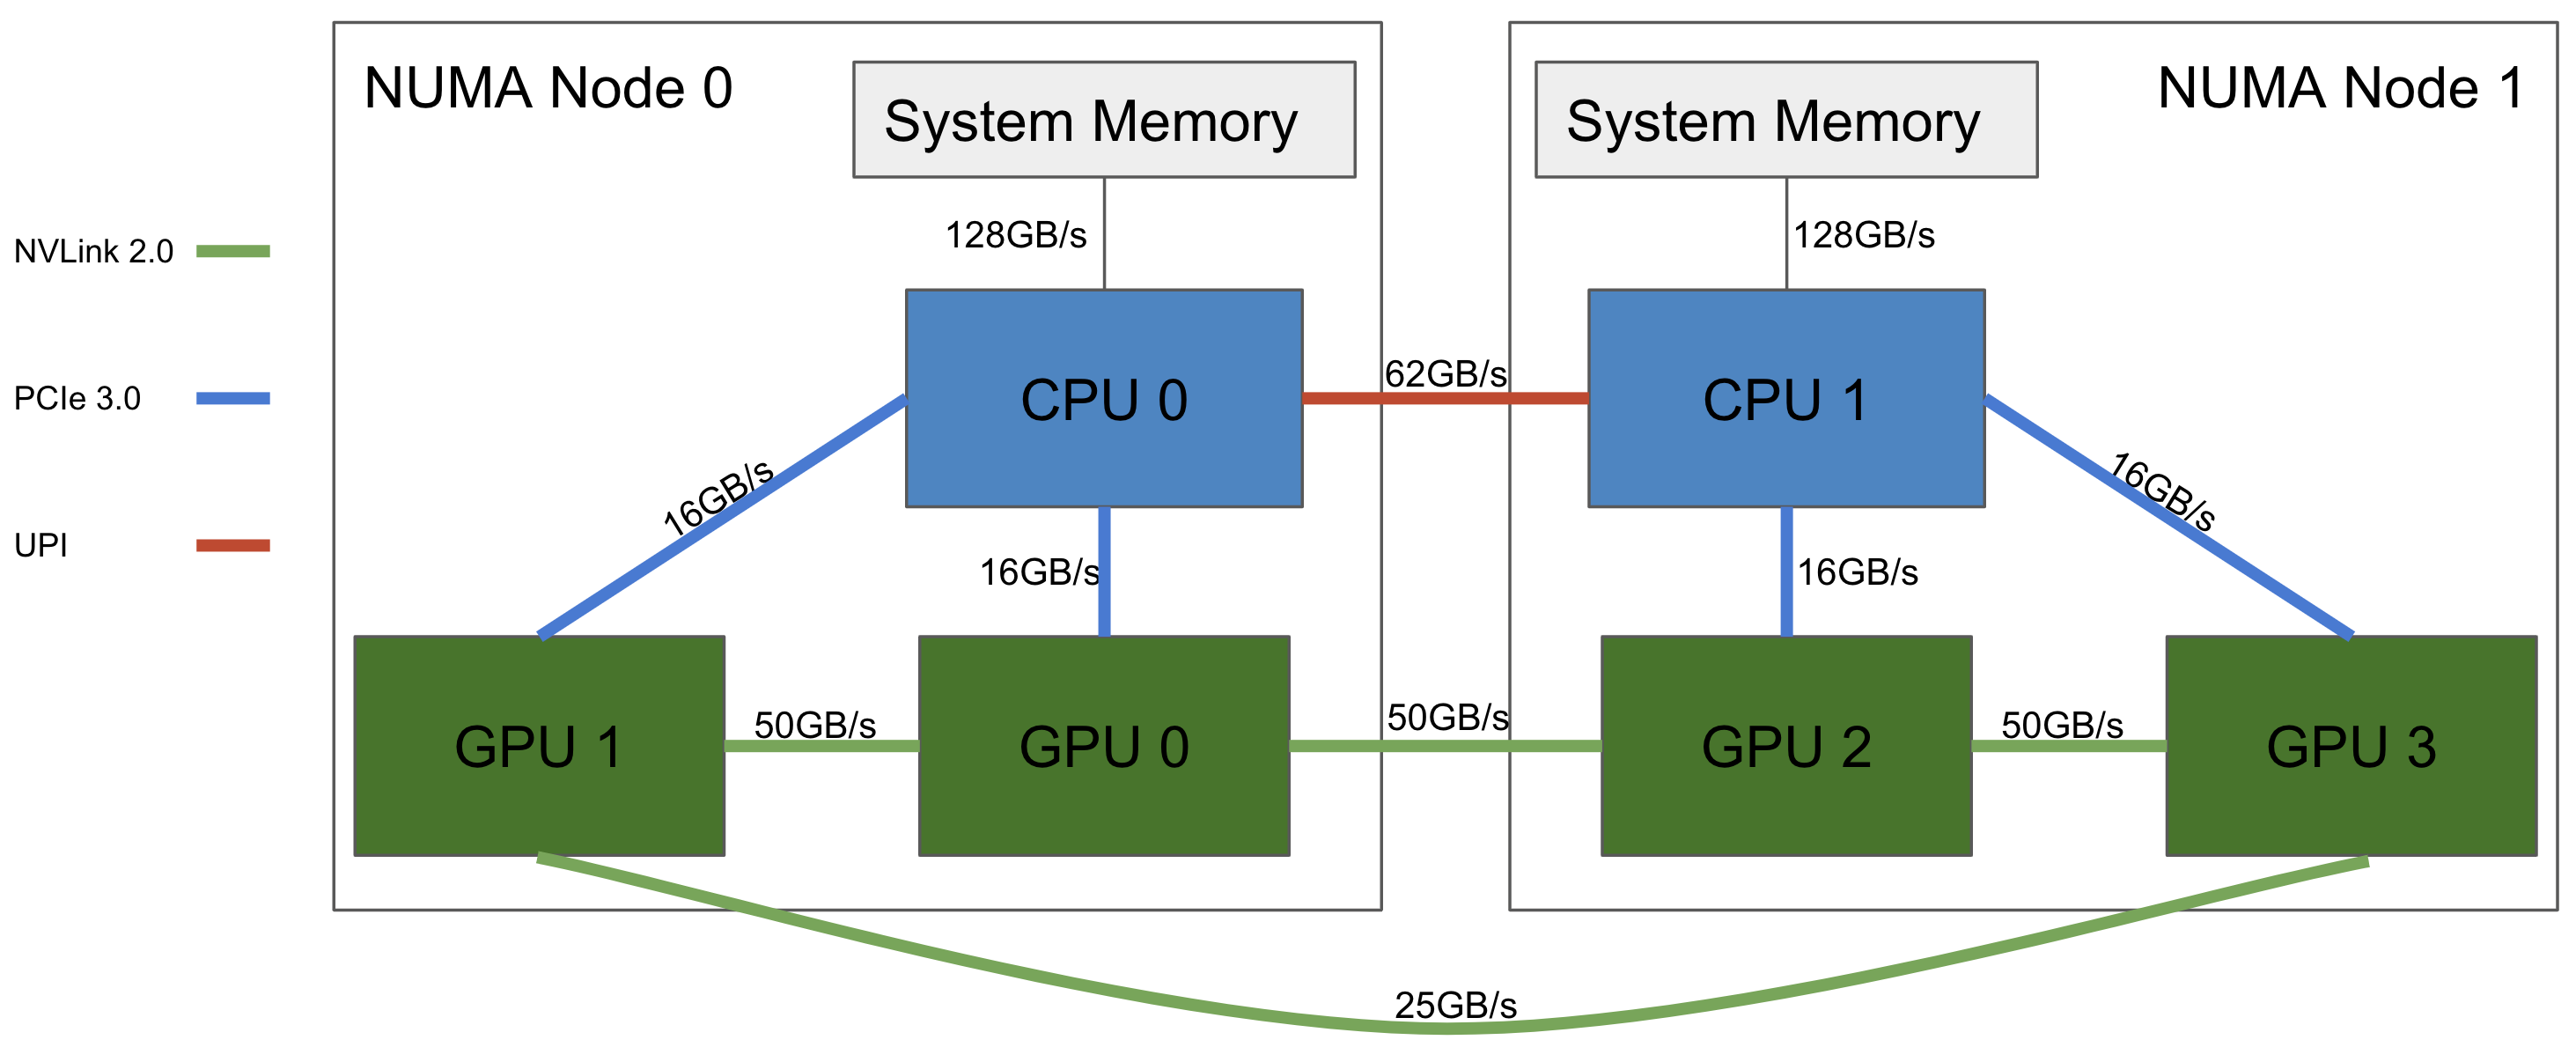
\includegraphics[width=\textwidth]{figures/delos_system_arch.png}
  \centering
  \label{fig:delos_arch}
\end{figure}

Two different systems are used for the evaluation. One system, which will be called Delos \ref{fig:delos_arch} in the following, consists of 4 Nvidia Tesla V100 GPUs with each 32GB of SXM2 memory and 2 Intel Xeon Gold 6148 CPUs with each 755GB of DDR4 memory. The Tesla V100 GPU clock rate is 1,53 GHz. It contains 80 Streaming Multiprocessors which each can execute a maximum of 2048 threads concurrently \cite{NVIDIATESLAV1002017}. The Intel Xeon Gold 6148 has 20 cores with a clock rate maximum of 3,70 GHz. Each core has two so-called hyper threads so that the CPU can execute 40 threads concurrently.

The second system, which will be called AC922 in the following, is a high-performance computing system developed in collaboration with IBM and Nvidia \cite{caldeiraIBMPowerSystem}. It incorporates the same GPUs as the Delos system (4xNvidia Tesla V100) and two IBM Power9 processors. Each Power9 processor has 16 cores with a clock rate maximum of 4 GHz, which, by using SMT4 multithreading, can execute 64 threads concurrently. 256GB DDR4 RAM is connected to each CPU.

Through the collaboration of IBM and Nvidia, the interconnect between a CPU and GPU in this system is NVLINK \cite{NVLink2021, zargesEvaluationOnNodeGPU} with a bandwidth of 150GB/s in contrast to the Delos PCIe 3.0 16GB/s interconnect. NVLINK is also faster latency wise \cite{liEvaluatingModernGPU2020}. The latency and throughput differences of both systems allow evaluating bottlenecks regarding interconnect speed in this heterogeneous computation scenario.
Furthermore the collaboration brings other features which a heterogeneous computing application can benefit from, such as Adress Translation Services \cite{ibmpower9nputeamFunctionalityPerformanceNVLink2018} unifying the GPU and CPU page table, native atomics support for system wide accessible memory and direct GPU memory access by the CPU \cite{UNIFIEDMEMORYP9}.

The following experiments only use one GPU for execution, even if the proposed algorithm can be executed on multiple GPUs at once. Therefore parameters, such as GPU-GPU memory handling and interconnect technology, do not influence the CPU-GPU computation results. Some benchmarks are pinned to the NUMA node closest to the executing GPU to limit interconnect effects not related to the direct CPU-GPU connection. Both systems' CPUs are each directly connected to two GPUs, whichs means using only half the cores and memory while NUMA pinned. The largest dataset being used with the size of 36GB$\sim$ will not be the limiting factor for the CPU's associated memory of 755GB on Delos and 256GB on AC922. On the other hand, 36GB$\sim$ of data will fill the GPU's memory of 32GB which is intentional behavior as said above.

The following table shows the tools and libraries used for the experiments:
\begin{table}[h!]
  \centering
  \begin{tabular}{||c | c||} 
   \hline
   Delos & AC922 \\ [0.5ex] 
   \hline\hline
   GCC 8.4.0 & GCC 8.3.1 \\
   CUDA 11.3 & CUDA 11.3 \\ 
   CMake 3.20.2 & CMake 3.20.2 \\
   Armadillo 10.5.1 & Armadillo 10.5.1 \\
   Boost 1.65.1 & Boost 1.76.0 \\ [1ex]
   \hline
  \end{tabular}
  \caption{Tools and libraries and their versions used in the experiments}
  \label{table:libversions}
\end{table}

Further the following flags were passed to GCC on the systems:
\begin{itemize}
  \item Delos: -O3 -DNDEBUG -march=native -mtune=native
  \item AC922: -O3 -DNDEBUG -flto -fpeel-loops -funroll-loops -ftree-vectorize -ffast-math -mcpu=power9 -mtune=power9
\end{itemize}
The flags used on the AC922 system are recommended by IBM for optimized binaries \cite{LinuxIBMPower}. NVCC, the Nvidia CUDA compiler, gets passed the same flags on both systems (-O3 -DNDEBUG -lineinfo) and additionally CMake autmatically sets the correct flags to compile for best optimization on the V100 architecture.

\section{Benchmarks}
For each system, basic experiments for both approaches are done first to determine the relevance and effectivness of those approaches. To analyze hardware-specific effects on the experiments, more detailed benchmarks are done later, such as tests with a modified thread count used for the CPU execution.
The first approach, which is called pre-balanced, will be tested and compared to the GPU only execution of the algorithm. Additionally, the effect of migrating edges after each level and pinning the execution to some NUMA node is tested as well.

The same tests are then done for the workstealing approach, where a test for atomic usage is added, since atomics are not necessary for this approach and only used so that edges are not processed twice.

Those described experiments are done on both the Delos system and the AC922 system. On the Delos system, further experiments to evaluate the scalability of the approaches are done using larger datasets as said above.

\subsection{Benchmarks Delos}
\begin{table}[H]
  \centering
  \begin{tabular}{||c | c | c | c||} 
   \hline
    & Execution time (ms) & $\Delta$ & $\Delta$ speedup in \% \\ [0.5ex] 
   \hline\hline
   GPU-only & 16290.8 & 0 & - \\
   Pre-Balanced & 15853.8 & -437 & 2,68 \\ 
   No post level migrations & 15821.8 & -469 & 2,96 \\
   NUMA node pinned & 16839.6 & 548,8 & -3,36 \\ [1ex] 
   \hline
  \end{tabular}
  \caption{Pre-Balanced execution time results (Delos)}
  \label{table:preb_delos}
\end{table}
The first experiments using the pre-balanced approach seen in \ref{table:preb_delos} show that there is a slight performance boost of 2,9\% in comparison to the GPU-only variant possible. While pinning the NUMA node, there is even a slow down seen, which tells us two things: First, the missing processing power of the lost cores while pinning the execution is missing, and more cores should help in speeding up the execution. Second, the interconnect bottleneck does not hit the performance in a meaningful way when edges of different rows are processed by GPU and CPU, supported by the little to no effect of migrating edges after level execution. Additionally, the count of rows placed on the CPU by the load balancer had to be tuned carefully for the best performance. The row count balanced on the CPU are in level one and two, 14 rows and in level three and four 8 rows, which is small compared to the maximum of 1000 rows.

This volatility does tuning the pre-balanced approach hard, especially for large datasets where the PC stable algorithm can execute for hours or even days. Multiple tuning executions might not be feasible in such situations, because this threshold might change alot for different datasets which could lead to more sparse rows.



\subsection{Benchmarks AC922}


% - Explain dataset used for testing (TCGA)
%   - Variable size
%   - how sampled
%   - paper (perscheid etc)
% - Show delos as a testing machine
%   - Intel Xeon 
%   - Nvidia  V100
%   - specs
%   - numa nodes
% - Show AC922
%   - Explain why power9 + V100 special
%   - ATS: Malloc is enough
%   - Faster interconnect NVLINK
%     - Comparison between interconnects
%   - Other pros : atomics etc
%   - Explain why this should affect my performance
%   - Compare Power9 to Intel Xeon
% - Show iteration measurements per level
%   - show how many tests and iterations have to be done

% - Measurements of GPU only Code

% - Measurements of Pre-balanced
%   - With, without migrating edges
%   - Different thresholds
%   - Different Dataset sizes
%   - Different omp scheduling methods
%   - Pinning on NUMA nodes
%   - Delos vs AC922
% - Measurements of Workstealing
%   - With, without migrating edges
%   - Different Dataset sizes
%   - Pinning on NUMA nodes
%   - Delos vs AC922

% - Measurements with different Datasets
%   - Iterations
%   - Workstealing Numa 0
%   - Prebalanced
%   - GPU only

	%!TEX root = ../thesis.tex
\chapter{Related Work}
\label{chap:relwork}
In this chapter related work that helped to build the heterogeneous computing approaches is looked into. Work that is relevant in the thesis context is elaborated and compared to the work done in this thesis.

In the context of Constraint Based Causal Structure Learning or more specifically the PC algorithm, there is related work with a focus on accelerating and improving the performance through utilization of the hardware. The most in-depth researched question is based on the general performance of CPU-based systems \cite{leFastPCAlgorithm2019, leParallelPCPackageEfficient2018, schmidtLoadBalancedParallelConstraintBased2019, colomboOrderIndependentConstraintBasedCausal,kalischEstimatingHighDimensionalDirected2007,scutariBayesianNetworkConstraintBased2017, madsenParallelAlgorithmBayesian2017,madsenParallelisationPCAlgorithm2015,nguyenMrPCCausalStructure2020}. 

Using the PC-stable variant of the PC algorithm by Colombo et al. \cite{colomboOrderIndependentConstraintBasedCausal}, Le et al. \cite{leFastPCAlgorithm2019, leParallelPCPackageEfficient2018} developed a modified PC-stable algorithm for parallel multi-core execution on the CPU by splitting each levels CI tests for an edge into tasks and process them in parallel. The algorithm is also called ParallelPC and as can be seen in the paper, does perform better than the single threaded PC-stable algorithm. The thesis CPU execution of both approaches follows this task split for aiming to get a similar parallelism speed. Both the papers and the thesis' versions are possible because of the order independence of the PC-stable algorithm.

While the tasks of the ParallelPC are statically scheduled onto the cores of the CPU, an imbalance can occur which is described in Schmidt et al. \cite{schmidtLoadBalancedParallelConstraintBased2019}. The load-balanced version of the PC-stable algorithm described in this paper uses a dynamic mapping technique to prevent an imbalanced execution. A central task queue is created in each level, where workers running on each core can take their next task and process that task. The thesis' CPU side execution uses OpenMP's possibility of dynamic task scheduling \cite{breshearsArtConcurrencyThread2009}. The workstealing approaches heterogeneous dynamic scheduling is based on the dynamic load-balancing idea of Schmidt et al. \cite{schmidtLoadBalancedParallelConstraintBased2019}, but avoids the task-queue's global system-wide singleton and introduces task specific synchronization primitives, to minimize communication between workers over the CPU-GPU interconnect.

Based on the work of the CPU based PC algorithm approaches, related work for a few GPU accelerated variants \cite{schmidtOrderIndependentConstraintBasedCausal2018,zarebavaniCuPCCUDAbasedParallel2018} exists. Both papers base their work on the PC algroithm described in Colombo et al. \cite{colomboOrderIndependentConstraintBasedCausal} where tasks are scheduled statically. The advantage of a GPU parallelized variant is, that the developer of the algroithm does not handle scheduling. The GPU runtime decides, how tasks are scheduled \cite{olmedoDissectingCUDAScheduling2020}. Using the GPU scheduler, all tasks are placed on the GPU and execution is handled by the GPU. The same approach is used in the GPU side execution of this thesis but in the pre-balanced approach some tasks are filtered before placing them on the GPU. In this thesis the implementation of Schmidt et al. \cite{schmidtOrderIndependentConstraintBasedCausal2018} is followed for the GPU side execution.

The related work for the PC algorithm is highly relevant to the work done in this thesis. The base implementation is heavily influenced by them and helped to form the heterogeneous computing variant.

For an entry into the heterogeneous computing topic surveys such as heterogeneous computing techniques by Mittal and Vetter \cite{mittalSurveyCPUGPUHeterogeneous2015}, where work for different scheduling techniques such as static and dynamic scheduling are introduced. Based on this, other related work can be found for a more detailed introduction into heterogeneous systems like Khokar et al. \cite{khokharHeterogeneousComputingChallenges1993} where Fosters' Methodology for parallel algorithm design is considered which is also used in this thesis and the heterogeneous computing environment impact is looked into. Parts of the scheduling, synchronization and interconnect thoughts of Khokar et al. \cite{khokharHeterogeneousComputingChallenges1993} influenced the thesis' approach and heterogeneous computing considerations.

In the paper by Carabano et al. \cite{carabanoExplorationHeterogeneousSystems2013}, differences between the CPU, GPU and other processing units, that are commonly used in hetterogeneous system, are elaborated and clarified. The main aspects of the CPU, which is said to used best on serial tasks, and the GPU, whichs properties are many aligned to parallelism, are further dealt with in this thesis. Such work supports the argumentation of both the GPUs and CPUs detailed properties, such as energy efficiency and performance, which are the basis of heterogeneous systems. With the broader look at CPU and GPU capabilities, a better scheduling can be achieved.

Zhang et al. \cite{zhangDynamicStaticLoad1991} and Topcuoglu et al. \cite{topcuogluPerformanceeffectiveLowcomplexityTask2002} explain the differences between static and dynamic scheduling, which formed the two different approaches based on those scheduling variants. Specifically in Zhang et al. \cite{zhangDynamicStaticLoad1991} dynamic and static scheduling and their effects in the context of NUMA shared memory multiprocessing is examined. The results of that analysis helped exploring effective scheduling strategies on heterogeneous NUMA systems and developing an effienect parallel program. The same obtained insights are made in both this thesis and the papers analysis, such as static scheduling is generally faster but has to be adjusted and dynamic scheduling while having the scheduling overhead, is more adaptble to the system.
The pre-balanced approach, which is inspried by static scheduling, does the balancing before level execution, but it still adds its overhead to the total execution time and the dynamic scheduling approach is therefore more promising.

In every heterogeneous computing, tasks have to be scheduled on different processing units, therefore related work based on the parallel task and tis load balancing in context of heterogeneous computing is also relevant for this thesis. There is work for the general view on the heterogeneous computing scheduling and load balancing topic \cite{cirouTripletClusteringScheduling2001, abdelkaderDynamicTaskScheduling2012,binottoDynamicReconfigurableLoadbalancing2010,galindoDynamicLoadBalancing2008,kopetzRealTimeScheduling1997,kwokStaticSchedulingAlgorithms1999,momcilovicDynamicLoadBalancing2014,singhSurveyStaticScheduling2015}. In the papers by Cirou et al. \cite{cirouTripletClusteringScheduling2001} and Abdelkader et al. \cite{abdelkaderDynamicTaskScheduling2012} dynamic task scheduling algorithms for hetergoeneous systems are explored. The Heterogeneous Earliest Finish Time (HEFT) and the Triplet clustering algorithm are two important algorithms in this topic, that both show promising results. Still for best performance results a domain specific parallelization developed for the PC-stable algorithm showed the best effect using a task length estimation by inspecting adjacency row lengths.

By inspecting the work on load balancing, the workstealing scheduler seemed best fitting for the PC algorithm use-case, next to the basic static scheduling (pre-balanced) approach. In literature about both dynamic and static scheduling, efficient algorithms are found for scheduling, that look into different factors of hetergeneous systems, where the utilization of the processing units is an important factor and helped forming both approaches aligned to the heterogeneous system requirement. 

Workstealing as a concept evolved from being used in CPU thread scheduling \cite{blumofeSchedulingMultithreadedComputations1999} into being relevant in parallel computing as well \cite{letzWorkStealingScheduler2010,mattheisWorkStealingStrategies2012,prellEmbracingExplicitCommunication2016}. As said in Blumofe et al. \cite{blumofeSchedulingMultithreadedComputations1999}, the workstealing scheduler reduces necessary communication, which limits the interconnect usage. The idea of the workstealing approach is based on this work.


	%!TEX root = ../thesis.tex
\chapter{Discussion}
\label{chap:discussion}
In this chapter, the results of the experiments in Chapter \ref{chap:experiments} are discussed. In the discussion, the results critic points are worked out. In the end, we answer the research question of the problem statement chapter \ref{chap:problem_statement}.

% Performance improvements could be shown for level 2 and 3
% But only in specific contexts
%   - doees not scale well
%   - perfect for situations, where the GPU gets to its (memory) limit
% 
As can be seen in Table \ref{table:ac922_vs_delos} performance improvements are achievable through introducing heterogeneous computing in the PC algorithm context. With a performance improvement of 16,5\% compared to the GPU-only variant, using the additional resources of the heterogeneous system is beneficial for the execution time.

With a deeper look into this performance by looking at the different levels in Figure \ref{fig:levelwise_delos} it is clear that the performance improvement is conditionally bound to the level and dataset used. The examination of the dataset solidifies this result in Chapter \ref{chap:est_speedup}. Estimating level-wise potential speedup shows that levels 3 and 4 tend to have the most and strongest outliers of maximum iteration counts. This is reflected by the level-wise tests, where level 3 shows the most speedup in Figure \ref{fig:levelwise_delos}, Figure \ref{fig:levelwise_ac922} and even clearer in Figure \ref{fig:levelwise_scaled_delos}.

The speedup estimation showed an even better potential speedup for the 4th level. The slowdown seen in the benchmarks can be explained by a very sparse adjacency matrix as a starting point to level 4. The execution time of that level is low, with around 200 milliseconds for the TCGA-1000 dataset. The low execution time leads to the overhead of introducing heterogeneous computing being higher than the benefits gained.

A preliminary speedup estimation analysis of the dataset could be beneficial for the heterogeneous computing approach and to decide which levels should be optimized using that method.

Solidifying the dataset and level dependency, using a 10 000 variables dataset slowed down the execution and only opened a performance improvement when looking at the level-wise performance. In level 3, the GPU-only variants execution duration is 2,467,224 ms, and the Delos workstealing execution duration is 2,107,416 ms.
The difference in level 3 is a 17,1\% improvement of performance by using both CPU and GPU. However, since every other level is slower with the workstealing execution, the whole execution time worsens. The 17,1\% performance improvement of level 3 is a solid increase, looking at the estimated possible speedup of around 30\%.

Level 2 is faster in the heterogeneous approach than in the GPU-only variant only for the 1000 variable dataset. There is a performance regression with the 10 000 variables dataset, hinting at a scaling problem.
This scaling issue is irrelevant as soon as the memory limit of the GPU is reached, at which the heterogeneous approach helps a lot with its 6,61x speedup in comparison to the GPU-only variant \ref{table:workst_delos_scaling}.

% Workstealing better than pre-balanced through dynamic nature
%   - does not have to be tuned
% Pre balanced is very hard to tune (might be even harder for different datasets)
%   - perforamnce characteristic has to be look at while tuning
%   - what is perforamnce? Too complex to decide. Just heuristics, which could not be portable to other systems
%   - The bigger the dataset, the worse to tune (long runtimes)
%   - Tuning after execution does not help, because the tuned values are not really reusable

\paragraph{Limitation of the Heterogeneous Approaches}

As outlined in the experiments chapter \ref{chap:experiments} tuning the load-balancer for the pre-balanced approach is necessary and non-trivial. The tuning problem could be handled by moving from balancing rows, whose execution time can vary greatly and is only approximately estimated, to single edges as tasks. The execution time of an edge as a task could still be estimated via the row length of the adjacency matrix this edge is on, but the run time impact of a single balanced task would be less. Therefore a more fine-grained balance would be achieved.

Still, tuning the parameters before execution leads to non-optimal balanced task distribution on CPU and GPU. For a better balance, multiple executions with different parameters approximate the best balance, or hardware performance characteristics are used for a better first execution balance. Multiple executions can be inefficient in real-world use cases, where the relevant result is already accessible after the first execution. Hardware characteristics, such as CPU performance, are hard to grasp with modern CPUs, where complex optimizations such as SIMD instruction set extensions and simultaneous multithreading (SMT) exist. Due to those optimizations, clock speed and core count of a CPU do not estimate the modern CPU's performance enough for smart load-balancing.

Due to the better execution times for single invocations and its hardware specification independence, the workstealing/dynamic scheduling approach is better suited for real-world use cases. Especially for large-scale datasets, where a single execution of the PC algorithm could run for days, the dynamic nature of the approach helps to optimize in the first run and therefore save time.

Disregarding the multithreading issues seen on the AC922 system, with a single thread of the CPU helping the heterogeneous computing variant, the execution does not seem very hardware reliant. Different CPUs with varying clock speeds and optimizations change the execution time results insignificantly. By looking at the fastest single-threaded workstealing experiments of both the Delos and the AC922 system, the AC922 single thread steals 108 edges in level 2 and 23 edges in level 3. In contrast, the single thread of the Delos steals 104 edges in level 2 and 25 edges in level 3. The execution times of both levels on both systems are nearly the same, with a deviation of around 40 ms.

Those single-threaded results also solidify that some multithreading issue is happening on the AC922 system, where additional threads slow the execution down. Since there should be a speedup by using more threads, this can be seen as a bug in the implementation and needs further investigation in future work. Fixing this bug could boost the AC922 experiment's performance and lead to even better performance results.

Both introduced approaches in this thesis use the resources of the underlying heterogeneous system and speed up the PC algorithms execution. Further improvements for optimizing the approaches are looked into in the following future work chapter. Therefore, the solution proposed seems promising for future heterogeneous computing efforts in the Constraint-Based Causal Structure Learning context.
% Hardware impacts execution times alot (SMT, difference AC922 vs Delos)
% Has to be decided for each system if applying is worth
% Multithreading not efficient (could be fixed)
% 
% 
% 
% Topic has to be further look into but seems promising
% 
% 
% 
	%!TEX root = ../thesis.tex
\chapter{Future Work}
\label{chap:fuwork}
This thesis experiments rely on the same dataset with different sized variable samples. Although this helps to get a first good impression on the effectiveness of the approaches, there is still a bias in the experiment result regarding the datasets structure and edge deletion behavior. If the edge deletion state of the graph is different, there is expected to be a different effectiveness outcome. While a more significant difference in outlier versus non-outlier task length could result in more effective outlier scheduling on the CPU, less to no outlier occurrence should make the GPU-only variant more effective.

This dataset behavior could be tested by executing the benchmarks with a different alpha value, directly influencing the amount with which edges are deleted. Another way of testing is generating datasets that show one of the said behaviors.

For better comparison, other real-world dataset experiments could be done. Multiple gene expression datasets are often used in the context of benchmarking the PC algorithm, such as NCI-60, MCC, or BR51 \cite{leFastPCAlgorithm2019}. By executing benchmarks with said datasets, direct comparisons to state-of-the-art methods could be made to understand the performance implications of both approaches better. Additionally, insights about the approaches dependency on the dataset and the effectiveness in other real-world cases can be derived.

The approaches shown in this thesis are not dependent on some specific CI-test. For simplicity, every benchmark was done using a CI-test that fits the multivariate normal distribution. For other distributions such as categorical data, other tests are used \cite{scutariLearningBayesianNetworks2010}. Those other tests require other data structures and can change the data access patterns significantly. With other data access patterns, the data dependencies between tasks change, and therefore, the interconnect usage between CPU and GPU has to be considered algorithm design-wise. Testing other CI-test could help to get insights on how those tests fit the heterogeneous computing setting.

Real-world datasets are not always composed of variables distributed in the same way. Mixed distribution datasets are also called heterogeneous datasets and require more complex conditional independence tests. Different CI-tests are possibly better executed on different specialized processing units. In heterogeneous datasets, a more complex load-balancing could be introduced that balances tasks also based on the CI-test used in this task.

The two used heterogeneous systems called Delos and AC922, the experiments are based on, show that the underlying system/hardware specifications are essential for the execution of heterogeneous computing. Other systems could be added to the experiments to understand the influences of the underlying hardware. Those systems could feature different performance disparities between CPU and GPU to get further insights into the effects of the hardware in contrast to the interconnect. Adding multiple GPU benchmarks could also be interesting to test and profile execution times. Sometimes two different system GPUs are directly connected to two different system CPUs. A more intelligent scheduling algorithm could be beneficial in such a system, identifying which task to steal from which GPU for best performance.

Heterogeneous systems do not only consist of CPUs and GPUs. Many different kinds of processing units could also support the algorithm execution. One of the also widely know processing units is called Field Programmable Gate Array (FPGA). FPGAs can be programmed to mimic a computer chip specifically designed for a purpose. The developer is in charge of deciding what gate is connected to which and designs hardware via software. An FPGA is more efficient in comparison to CPU and GPU when used correctly, \cite{qasaimehComparingEnergyEfficiency2019} and could be added to the heterogeneous computing solution proposed in this thesis to accelerate further.
% Test with different dataset charateristics
% Test with Stronger CPU/GPU disparity
% Add FPGA
% 
	\clearpage
	%\printglossary[type=\acronymtype],style=modsuper]
	\bibliography{Remote}
%	\begin{appendices}
%	%!TEX root = ../thesis.tex
\chapter{Appendix}

%	\end{appendices}
	%!TEX root = thesis.tex
\selectlanguage{german}
\chapter*{Eigenst"andigkeitserkl"arung}
Ich erkl"are hiermit, dass ich die vorliegende Arbeit selbst"andig verfasst und keine anderen als die genannten Quellen und Hilfsmittel verwendet habe.
\\
\\
\\
\\
\\
Potsdam, \today
\\
\\
\\
\\
\AUTHOR

\end{document}
